\documentclass[natbib,twocolumn,twoside]{svmultiag}
%
%\usepackage[dvips]{graphicx}
\usepackage{graphicx}

% Extra packages
\usepackage{amsmath}
\usepackage{xcolor}
\usepackage{multirow}
\usepackage{tabularx}
\newcolumntype{C}{>{\centering\arraybackslash}X}

% ============================================================================
\graphicspath{{./figures/}}

\title*{Where -- A New Software for Geodetic Analysis}
\titlerunning{Where -- A New Software for Geodetic Analysis}

\author{A.-S. Kirkvik, G.A. Hjelle, M. D\"ahnn, I. Fausk, E. Mysen}
\authorrunning{Kirkvik et al.}

\institute{Ann-Silje Kirkvik, Geir Arne Hjelle, Michael D\"ahnn, Ingrid Fausk,
  Eirik Mysen \at Norwegian Mapping Authority, Geodetic Institute,
  Kartverksveien 21, 3511 H{\o}nefoss, Norway
}
% ============================================================================
\begin{document}
\maketitle
% ----------------------------------------------------------------------------
\abstract{%
At the Norwegian Mapping Authority we are currently developing Where, a new
software for geodetic analysis. Where is built on our experiences with the
GEOSAT software, and will be able to analyse data from geodetic techniques such
as VLBI, SLR and GNSS. The software is mainly written in Python. The code is
quick to write and the architecture is easily extendable and maintainable, while
at the same time taking advantage of well-tested libraries like the SOFA and
IERS packages. At the moment the VLBI analysis is close to ready. Comparison to
other softwares show that theoretical delay computations in Where are consistent
with those. Development of SLR and GNSS analysis is well under way, while DORIS
is postponed.
}

\keywords{VLBI, Python, Where, Software, VASCC, Comparison}


% ----------------------------------------------------------------------------
\section{Introduction}                                \label{sec:introduction}
% ----------------------------------------------------------------------------
Where is a new software for geodetic analysis, currently being developed at the
Norwegian Mapping Authority. Where is based on experiences from working with the
GEOSAT software~\citep{kierulf2010}, and is intended to be able to analyse data
from multiple space geodetic techniques used in the creation of reference
frames.

The last decade the Norwegian Mapping Authority has increased its contributions
to global reference frames. Currently, a new fundamental station is being built
at Ny-{\AA}lesund with VLBI, SLR, GNSS and DORIS. The Norwegian Mapping
Authority has also contributed to passing a UN resolution on global geodesy and
the importance of Global Geodetic Reference Frames\footnote{URL
  \texttt{ggim.un.org/UN\_GGIM\_wg1.html}}. The Where project is the third leg
in this effort, developing a new tool for the analysis of space geodetic data.

Full VLBI analysis of daily sessions will soon be possible with Where and this
paper will briefly explain the implementation strategy in Where. Some results
from tests to verify the implementation of the theoretical model will be
shown. Finally, an outline of the remaining activities to complete the VLBI
pipeline is presented. Analysis of SLR and GNSS is in development, while
DORIS analysis is postponed.


\section{Architecture}

Where is mainly implemented in Python. The Python ecosystem for data science is
very rich and powerful. Python is Open Source and freely available on all major
platforms\footnote{URL \texttt{python.org}}. In addition, Python smoothly
interfaces with other languages like C and Fortran, which allows Where to use
the \texttt{SOFA}\footnote{URL \texttt{iausofa.org}\label{ft:sofa}} and
\texttt{IERS}~\citep{iers_software} Fortran libraries directly. Python also
provides a comprehensive set of libraries. Where utilizes several well known
packages such as \texttt{numpy}\footnote{URL \texttt{numpy.org}},
\texttt{scipy}\footnote{URL \texttt{scipy.org}}, and
\texttt{matplotlib}\footnote{URL \texttt{matplotlib.org}} as well as more
specialized packages like \texttt{astropy}~\citep{astropy2013},
\texttt{pint}\footnote{URL \texttt{pint.readthedocs.io}} and
\texttt{jplephem}\footnote{URL
  \texttt{pypi.python.org/pypi/jplephem}\label{ft:jplephem}}.

Where stores the analysis output in HDF5\footnote{URL \texttt{hdfgroup.org}} and
JSON\footnote{URL \texttt{json.org}} files.  To explore the output a simple
graphical interface called There based on \texttt{matplotlib} is also being
developed. A screen-shot from There is shown in Figure~\ref{fig:there}.

\begin{figure}[tb]
  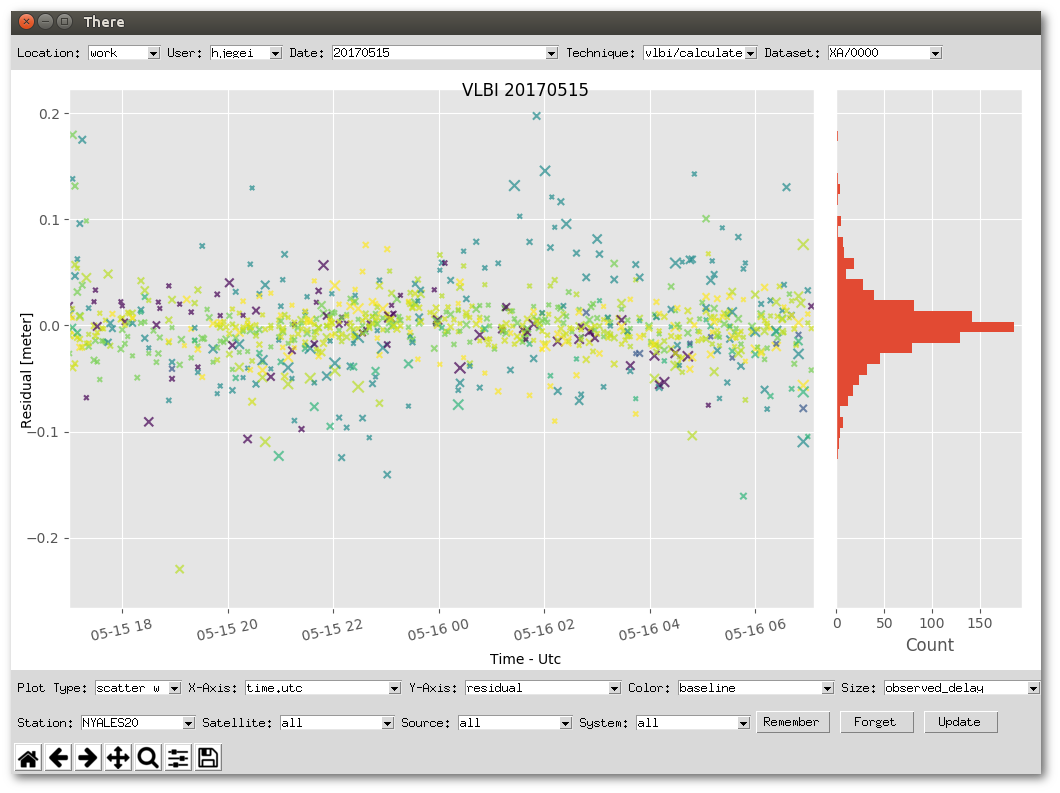
\includegraphics[width=\columnwidth]{kirkvik_fig01}
  \caption{A screen-shot of There. There is a graphical tool developed to look
    into the results and analysis done by Where.}
  \label{fig:there}
\end{figure}

Where works on the basis of a pipeline that is split into several stages, see
Figure~\ref{fig:architecture}. First, observation files are processed in the
\emph{read} stage and converted to an internal Where data structure. Next, in
the \emph{edit} stage bad observations are discarded and other filters such as
an elevation cut off angle can be applied. Next, theoretical delays are
calculated and a quadratic clock polynomial is estimated in the \emph{calculate}
stage. At this stage the analyst can inspect the residuals to identify for
instance clock breaks and bad cable calibration data and update the
configuration file for the edit stage accordingly. The \emph{edit} and
\emph{calculate} stage needs to be run again if any changes are made. Next,
station positions and other target parameters such as Earth orientation
parameters can then be estimated in the \emph{estimate} stage. Finally, results
are written to disk in proper formats in the \emph{write} stage.

\begin{figure}[tb]
  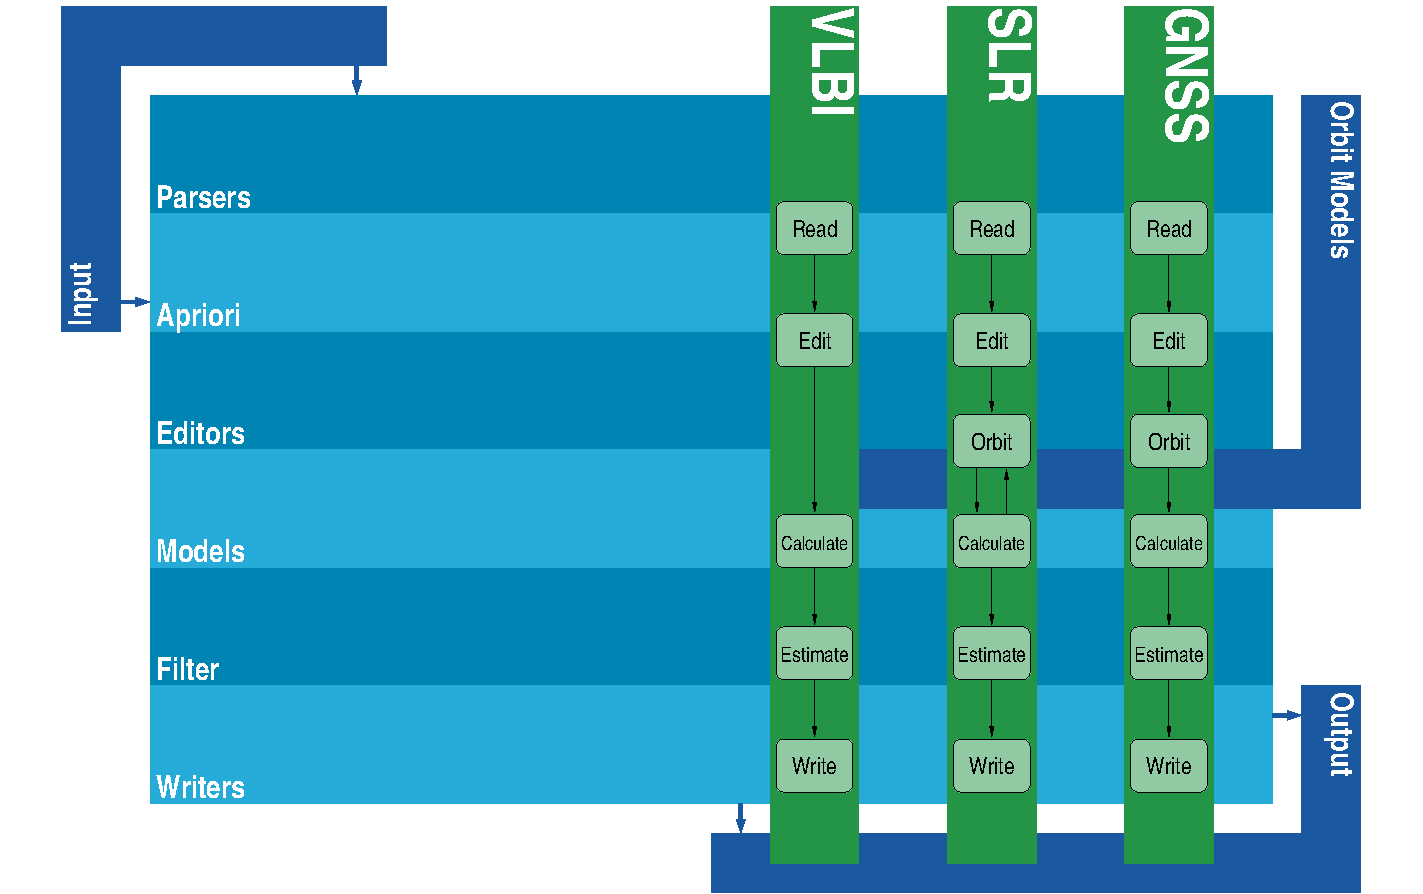
\includegraphics[width=\columnwidth]{kirkvik_fig02}
  \caption{An overview of the architecture of Where. Pipelines for the analysis
    of the different techniques is shown as vertical bars. Horisontal lines
    represent packages that to some extent can be reused across techniques.}
  \label{fig:architecture}
\end{figure}


\begin{table*}[t]
\begin{tabularx}{\textwidth}{r|X}
  \textcolor{black!99}{EOP}
    & \textcolor{black!99}{Lagrange interpolated C04 time series with
                           corrections for high frequency ocean tides and
                           liberations} \\
\textcolor{black!60}{Reference frames}
    & \textcolor{black!60}{ITRF2008/2014 (no post-seismic deformations) and ICRF2} \\
  \textcolor{black!99}{Ephemerides}
    & \textcolor{black!99}{DE405, DE421, DE430} \\
  \textcolor{black!60}{Displacement models}
    & \textcolor{black!60}{Atmospheric pressure loading, Eccentricity vector,
                           Ocean tidal loading, Ocean pole tides, Solid Earth
                           tides, Solid Earth pole tides} \\
  \textcolor{black!99}{Troposphere}
    & \textcolor{black!99}{GMF, GPT, GPT2, GPT2w, VMF1} \\
  \textcolor{black!60}{VLBI models}
    & \textcolor{black!60}{Axis offset, Cable calibration, Geometric and
                           gravitational delay, Ionosphere, Thermal
                           deformation} \\
  \textcolor{black!99}{Estimation}
    & \textcolor{black!99}{Kalman Filter with continuous piece-wise linear
                           functions} \\
  \textcolor{black!60}{Partial derivatives}
    & \textcolor{black!60}{Clock, Polar motion and rate, $\Delta$UT1 and rate,
                           Celestial pole offset, Source coordinates, Station
                           position, Zenith wet delay, Horizontal gradients} \\
\end{tabularx}
\caption{VLBI Models and apriori data supported by Where. A configuration file
  is used to choose between the different options.}
\label{tbl:models}
\end{table*}


\section{Implementation}

A VLBI model consistent with current conventions is fully implemented. In Where,
the theoretical delay $\tau$ is calculated according to
\begin{align}
  \nonumber \tau =& \tau_{\text{geom}} + \tau_{\text{grav}} + \Delta\tau_{\text{tropo}}
                    + \Delta\tau_{\text{axis}} - \\
                  & \Delta\tau_{\text{therm}} + \tau_{\text{clock}}
                    - \Delta\tau_{\text{cable}} + \tau_{\text{iono}} ,
  \label{eq:theoretical_delay}
\end{align}

\noindent with the notation
\begin{equation}
  \Delta\tau_{x} = \tau_{x}(\text{station}_2) - \tau_{x}(\text{station}_1) .
\end{equation}

\noindent The geometric and gravitational delays $\tau_\text{{geom}}$ and
$\tau_\text{{grav}}$ follow the consensus model in chapter 11 of the 2010 IERS
Conventions~\citep{iers2010}. The geocentric velocity of a receiver, $w_i$, in
the consensus model is implemented as
\begin{equation}
  w_i(t) = Q(t) \dot{R}(t) W(t) x_i
\end{equation}

\noindent where $t$ is the epoch of the observation. Furthermore, $Q(t)$, $R(t)$
and $W(t)$ are the transformation matrices discussed in chapter 5 of the 2010
IERS Conventions~\citep{iers2010} and $\dot{R}(t)$ is the time derivative of
$R(t)$. Finally, $x_i$ is the coordinate of the receiver in a terrestrial
reference frame.

Gravitational delays are included for the Sun, the Earth, the Moon, Mercury,
Venus, Mars, Jupiter, Saturn, Uranus, Neptune and Pluto. The planet ephemerides
are calculated using the Python package
\texttt{jplephem}\textsuperscript{\ref{ft:jplephem}} which reads the Satellite
Planet Kernel files provided by JPL and computes three-dimensional positions and
velocities for the planets.

The tropospheric delay $\tau_{\text{tropo}}$ is implemented according to chapter
9 in the 2010 IERS Conventions~\citep{iers2010} with VMF1~\citep{boehm2006a}
as default mapping functions. When available, routines from
\texttt{IERS}~\citep{iers_software} are used to calculate the delay due to the
troposphere.

The delays due to axis offset $\tau_{\text{axis}}$ and thermal deformation
$\tau_{\text{therm}}$ are implemented based on~\citep{nothnagel2009}. To account
for the time delay in the thermal deformation model a sine function is fitted to
the temperature data to estimate the temperature at 2 and 6 hours before the
observation epochs. The elevation angle is not corrected for refractivity, and
antennas with a radome are not treated differently than those without.

The ionospheric delay $\tau_{\text{iono}}$ and cable delay $\tau_{\text{cable}}$
are used directly as provided on the observation file. The delay due to clock
synchronization issues $\tau_{\text{clock}}$ is an estimated second degree
polynomial for all stations except one station that is kept fixed as a reference
station.

The apriori station coordinates are projected to the observation epochs using
the linear model provided with the reference frame. The station displacement
models from chapter 7 in the IERS Conventions 2010 are then applied to model the
variations in the station coordinates during the observation
period. Table~\ref{tbl:models} gives an overview of the models currently
available for Where. The station displacement models are based on the
\texttt{IERS}~\citep{iers_software} routines that are available.

The transformation between a terrestrial reference frame and a geocentric
celestial frame is implemented using
\texttt{SOFA}\textsuperscript{\ref{ft:sofa}} routines. The applied method is IAU
2006/2000A, CIO based using the X, Y series as described in section 5.6 in SOFA
Tools for Earth Attitude~\citep{sofa_tools}. The Earth orientation parameters
are interpolated to the observation epochs and corrected for ocean tides and
liberations using \texttt{IERS}~\citep{iers_software} routines as described in
chapter 5 of the 2010 IERS Conventions~\citep{iers2010}.

To handle the various time scales needed in a typical VLBI analysis, Where
utilizes the \texttt{Time} class of the \texttt{astropy}
library~\citep{astropy2013}. However, to ensure consistency, the transition
between UT1 and UTC is overridden by a custom implementation based on the
apriori UT1-UTC time series. Likewise, the transition between TT and TDB is
overridden by the method and software described in chapter 10 of the 2010 IERS
Conventions~\citep{iers2010}. For now, all the delay models and station
displacement models are calculated using the arrival time at the first station of
a baseline.

The estimation is done using a Kalman filter with a Modified Bryson-Frazier
smoother~\citep{bierman2006}. Currently, the clock errors and troposphere (wet
delay and gradients) are modeled using continuous piece-wise linear
functions. The Kalman filter solution is converted to reduced normal equations
using results from~\citep{mysen2017}. Table~\ref{tbl:models} summarizes the
parameters that can be estimated.

% ---------------------------------------------------------------------------
\section{Test results}
% ---------------------------------------------------------------------------
In 2015/2016 Grzegorz Klopotek at Chalmers University of Technology in Sweden
carried out a VLBI Analysis Software Comparison Campaign (VASCC). The goal of
the campaign was to compare computed theoretical delays from different software
packages. In total 11 different software packages contributed to the campaign
and the results where presented at the IVS General Meeting in South Africa in
2016~\citep{klopotek2016}.

The Norwegian Mapping Authority provided solutions to VASCC using the legacy
software GEOSAT~\citep{kierulf2010}. However, as development of the new software
progressed a new VASCC solution using Where was computed. This solution was
compared with VASCC solutions from the software packages
c5++~\citep{hobiger2010} and VieVS~\citep{boehm2012}.

The VASCC data-set includes two networks of stations: one with four stations on
the southern hemisphere (SH) and one with five stations on the northern
hemisphere (NH).  Virtual observations of one radio source for each network are
scheduled every minute for 15 days, from June 22nd to July 7th 2015. This
yielded a total number of 129600 observations for the southern network and
216000 observations for the northern network. A leap second is introduced at
midnight June 30th.

Not all terms of the theoretical delay~\eqref{eq:theoretical_delay} are included
in the campaign. The VASCC delay model includes geometric and gravitational
delay from the IERS 2010 Conventions~\citep{iers2010}. Also the delay through
the troposphere~\citep{iers2010} (hydrostatic delay with GMF mapping function)
and delay due to thermal deformations (with constant temperatures) and axis
offset as described by~\citep{nothnagel2009} are included. Delays due to cable
calibration, the ionosphere and clocks are ignored. Site displacement models
includes solid Earth tides, solid Earth pole tides, ocean tidal loading
(FES2004) and ocean loading pole tides according to~\citep{iers2010}. The
version of the IERS Conventional mean pole model used in VASCC is
2010. Atmospheric pressure loading and eccentricity vectors are ignored. The
apriori EOP time series is corrected for ocean tides and liberation effects with
periods less than two days according to~\citep{iers2010}.

\begin{figure}[tb]
  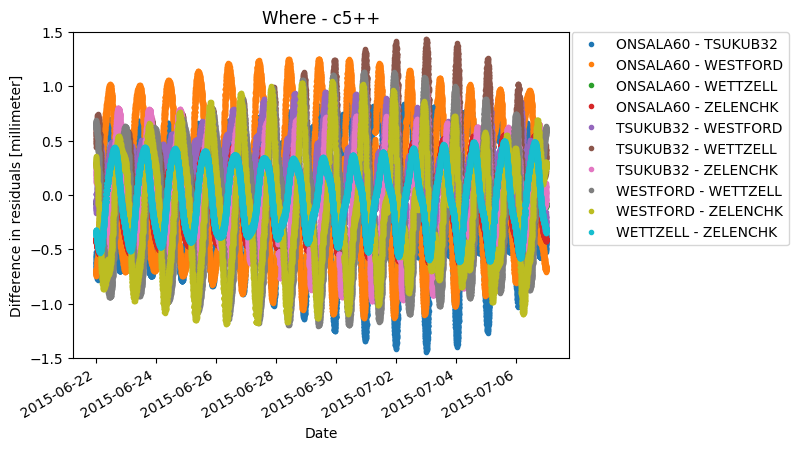
\includegraphics[width=\columnwidth]{kirkvik_fig03}
  \caption{Difference in theoretical delay between Where and c5++ for each
    baseline in the northern network used in the VASCC. The RMS of all
    differences is 0.49~mm.}
  \label{fig:where_c5++_sh}
\end{figure}

\begin{figure}[tb]
  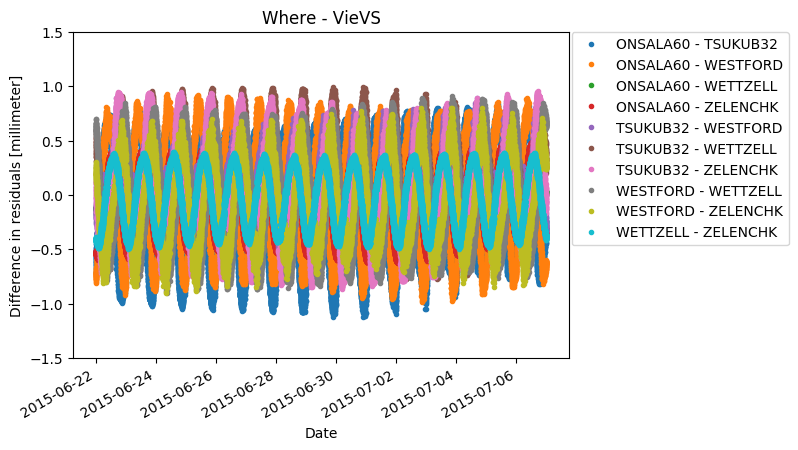
\includegraphics[width=\columnwidth]{kirkvik_fig04}
  \caption{Difference in theoretical delay between Where and VieVS for each
    baseline in the northern network used in the VASCC. The RMS of all
    differences is 0.44~mm.}
  \label{fig:where_vievs_sh}
\end{figure}

\begin{figure}[tb]
  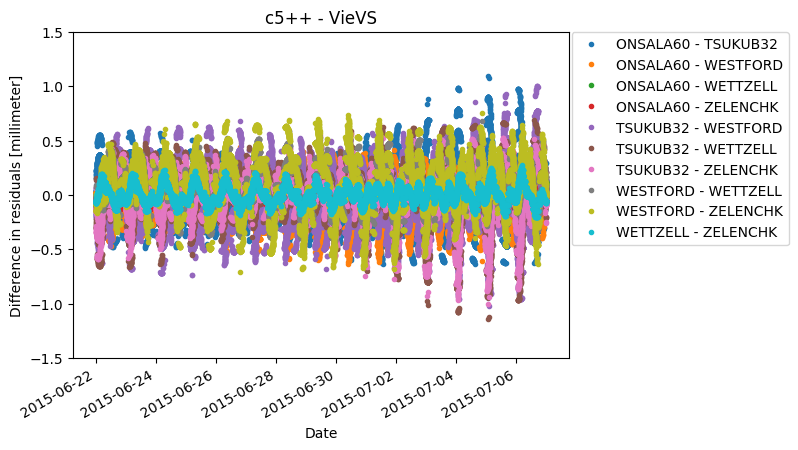
\includegraphics[width=\columnwidth]{kirkvik_fig05}
  \caption{Difference in theoretical delay between c5++ and VieVS for each
    baseline in the northern network used in the VASCC. The RMS of all
    differences is 0.21~mm.}
  \label{fig:c5++_vievs_sh}
\end{figure}

In the original campaign six software packages got sub-millimeter agreement when
comparing the RMS of the difference in theoretical delays for both networks
together over the whole period. The largest RMS difference between two of these
software packages was 0.71~mm and the smallest difference was 0.17~mm. The
absolute value of the largest difference in residual among these packages was
2.68~mm and the smallest difference was 0.83~mm. The solutions from two of the
these six software packages, c5++~\citep{hobiger2010} and
VieVS~\citep{boehm2012}, were compared with Where and the results are summarized
in Tables~\ref{tbl:vascc_rms}
and~\ref{tbl:vascc_max}. Figures~\ref{fig:where_c5++_sh},
\ref{fig:where_vievs_sh} and~\ref{fig:c5++_vievs_sh} show the difference between
Where, c5++ and VieVS for the northern network. For the southern network the
differences in residuals are slightly smaller.

\begin{table}
\renewcommand{\arraystretch}{1.2}
\begin{tabularx}{\columnwidth}{lrCCC}
  &       & \multicolumn{3}{c}{NH}   \\ \cline{3-5}
  &       & \textbf{Where}  & \textbf{c5++}   & \textbf{VieVS}  \\
  \multirow{3}{*}{\rotatebox[origin=c]{90}{SH}}
    & \multicolumn{1}{|l}{\textbf{Where}} & $\diamond$ &     $0.49$ &     $0.44$ \\
    & \multicolumn{1}{|l}{\textbf{c5++}}  &     $0.18$ & $\diamond$ &     $0.21$ \\
    & \multicolumn{1}{|l}{\textbf{VieVS}} &     $0.43$ &     $0.39$ & $\diamond$ \\
\end{tabularx}
\caption{RMS of difference [mm] between Where, c5++ and VieVS for
  the northern (NH, above diagonal) and southern (SH, below diagonal) network}
\label{tbl:vascc_rms}
\end{table}

\begin{table}
\renewcommand{\arraystretch}{1.2}
\begin{tabularx}{\columnwidth}{lrCCC}
  &       & \multicolumn{3}{c}{NH}   \\ \cline{3-5}
  &       & \textbf{Where}  & \textbf{c5++}   & \textbf{VieVS}  \\
  \multirow{3}{*}{\rotatebox[origin=c]{90}{SH}}
    & \multicolumn{1}{|l}{\textbf{Where}} & $\diamond$ &     $1.44$ &     $1.12$ \\
    & \multicolumn{1}{|l}{\textbf{c5++}}  &     $0.63$ & $\diamond$ &     $1.14$ \\
    & \multicolumn{1}{|l}{\textbf{VieVS}} &     $1.28$ &     $1.09$ & $\diamond$ \\
\end{tabularx}
\caption{Maximum absolute difference [mm] between Where, c5++ and
  VieVS for the northern (NH, above diagonal) and southern (SH, below diagonal) network}
\label{tbl:vascc_max}
\end{table}


% ---------------------------------------------------------------------------
\section{Conclusions and future work}
% ---------------------------------------------------------------------------
The comparison with the VASCC results indicate that the VLBI delay model in
Where is consistent with existing software packages and current conventions. The
VASCC data-set has been valuable in the development and testing of Where. An
extension of the campaign to include for instance the VMF1 mapping function and
partial derivatives is encouraged.

The \emph{estimation} and \emph{write} stages in Where are implemented, but some
testing remains. Where can read both \texttt{NGS} and \texttt{vgosDb} files, but
requires that the ionosphere and ambiguities are provided in the observation
files.

The Norwegian Mapping Authority is an associated analysis center within the IVS
and the short term plan is to finish a stable version of Where capable of
producing normal equations that can be used for IVS products~\citep{ivs}.
Additionally, the short term plan is to implement support for the post-seismic
deformation models in ITRF2014~\citep{itrf2014}.

The next step is to combine solutions from individual sessions to investigate
the behavior of for instance station coordinates over time. This work is
intended to monitor and ensure good data quality from the new antennas at
Ny-{\AA}lesund. Later, we will investigate the possibilities for solving the
ionosphere and ambiguities in the next step towards creating an independent
analysis software.

% ---------------------------------------------------------------------------
\begin{thebibliography}{10}
\providecommand{\natexlab}[1]{#1}
\providecommand{\url}[1]{\texttt{#1}}
\expandafter\ifx\csname urlstyle\endcsname\relax
  \providecommand{\doi}[1]{doi: #1}\else
  \providecommand{\doi}{doi: \begingroup \urlstyle{rm}\Url}\fi

\bibitem[Altamimi et~al.(2016) Altamimi, Z., P. Rebischung, L. Métivier, and C. Xavier]{itrf2014}
Z. Altamimi, et~al.
\newblock ITRF2014: A new release of the International Terrestrial Reference Frame modeling nonlinear station motions.
\newblock \emph{Journal of Geophysical Research: Solid Earth}, 121, pages 6109–-6131.
\newblock \doi{10.1002/2016JB013098}

\bibitem[{Astropy Collaboration} et~al.(2013){Astropy Collaboration},
  Robitaille, Tollerud, Greenfield, Droettboom, Bray, Aldcroft, Davis,
  Ginsburg, Price-Whelan, Kerzendorf, Conley, Crighton, Barbary, Muna,
  Ferguson, Grollier, Parikh, Nair, Unther, Deil, Woillez, Conseil, Kramer,
  Turner, Singer, Fox, Weaver, Zabalza, Edwards, Azalee~Bostroem, Burke, Casey,
  Crawford, Dencheva, Ely, Jenness, Labrie, Lim, Pierfederici, Pontzen, Ptak,
  Refsdal, Servillat, and Streicher]{astropy2013}
{Astropy Collaboration}, et~al.
\newblock Astropy: A community python package for astronomy.
\newblock \emph{Astronomy \& Astrophysics}, 558:\penalty0 A33, Oct. 2013.
\newblock \doi{10.1051/0004-6361/201322068}.
\newblock URL \url{www.astropy.org}.

\bibitem[Behrend(2013)]{ivs}
D. Behrend
\newblock Data Handling within the International VLBI Service
\newblock \emph{Data Science Journal} Vol. 12, pp. WDS81-–WDS84, ISSN 1683-1470, 17 Feb. 2013.
\newblock \doi{10.2481/dsj.WDS-011}

\bibitem[B\"ohm et~al.(2006)B\"ohm, Werl, Schuh]{boehm2006a}
J.~B\"ohm, et~al.
\newblock Troposphere mapping functions for GPS and VLBI from ECMWF operational analysis data.
\newblock \emph{GPS Solutions}, vol. 11, number B02406, 2006.
\newblock \doi{10.1029/2005JB003629}

\bibitem[B\"ohm et~al.(2012)B\"ohm, B\"ohm, Nilsson, Pany, Plank, Spicakova,
  Teke, and Schuh]{boehm2012}
J.~B\"ohm, et~al.
\newblock The new {V}ienna {VLBI} software {VieVS}.
\newblock In S.~Kenyon, M.~C. Pacino, and U.~Marti, editors, \emph{Geodesy for
  Planet Earth: Proceedings of the 2009 IAG Symposium, Buenos Aires, Argentina,
  31 August 31 - 4 September 2009}, pages 1007--1011, Berlin, Heidelberg, 2012.
  Springer Berlin Heidelberg.
\newblock \doi{10.1007/978-3-642-20338-1\_126}.

\bibitem[Bierman(2006)]{bierman2006}
G.J.~Bierman.
\newblock \emph{Factorization Methods for Discrete Sequential Estimation}.
\newblock Dover publications. 2006.
\newblock ISBN 9780486449814

\bibitem[Hobiger et~al.(2010)Hobiger, Otsubo, Sekido, Gotoh, Kubooka, and
  Takiguchi]{hobiger2010}
T.~Hobiger, et~al.
\newblock Fully automated {VLBI} analysis with c5++ for ultra-rapid
  determination of {UT1}.
\newblock \emph{Earth, Planets and Space}, 62\penalty0 (12):\penalty0 933--937, 2010.
\newblock \doi{10.5047/eps.2010.11.008}.

\bibitem[{IAU SOFA Tools}()]{sofa_tools}
{IAU SOFA Board}.
\newblock {SOFA} Tools for Earth Attitude.
\newblock URL \url{http://www.iausofa.org/publications/sofa\_pn.pdf}

\bibitem[{IERS contributors}()]{iers_software}
{IERS contributors}.
\newblock {IERS} software collection.
\newblock URL \url{ftp://maia.usno.navy.mil/conventions/2010}.

\bibitem[Kierulf et~al.(2010)Kierulf, Andersen, Boeckmann, and
  Kristiansen]{kierulf2010}
H.~P. Kierulf, et~al.
\newblock {VLBI} analysis with the multi-technique software {GEOSAT}.
\newblock In D.~Behrend and K.~D. Baver, editors, \emph{VLBI2010: From Vision
  to Reality}, volume NASA/CP-2010-215864 of \emph{IVS General Meeting
  Proceedings}, pages 207--211. IVS, 2010.
\newblock URL \url{ivscc.gsfc.nasa.gov/publications/gm2010/kierulf.pdf}.

\bibitem[Klopotek et~al.(2016)Klopotek, Artz, Bellanger, Bourda, Gerstl,
  Gordon, Haas, Halsig, Hjelle, Hobiger, Hugentobler, Iddink, Kirkvik, Lambert,
  Plank, Schmid, Shu, Titov, Tong, Wang, Xu, and Zheng]{klopotek2016}
G.~Klopotek, et~al.
\newblock Results from the {VLBI} analysis software comparison campaign 2015.
\newblock In D.~Behrend, K.~D. Baver, and K.~L. Armstrong, editors, \emph{New
  Horizons with VGOS}, volume NASA/CP-2016-219016 of \emph{IVS General Meeting
  Proceedings}, pages 203--207. IVS, 2016.
\newblock URL \url{ftp://ivscc.gsfc.nasa.gov/pub/general-meeting/2016/pdf/042\_klopotek\_etal.pdf}.

\bibitem[Mysen(2017)]{mysen2017}
E.~Mysen.
\newblock On the equivalence of {K}alman filtering and least-squares  estimation.
\newblock \emph{Journal of Geodesy}, 91\penalty0 (1):\penalty0 41--52, 2017.
\newblock \doi{10.1007/s00190-016-0936-3}.

\bibitem[Nothnagel(2009)]{nothnagel2009}
A.~Nothnagel.
\newblock Conventions on thermal expansion modelling of radio telescopes for
  geodetic and astrometric {VLBI}.
\newblock \emph{Journal of Geodesy}, 83\penalty0 (8):\penalty0 787--792, 2009.
\newblock \doi{10.1007/s00190-008-0284-z}.

\bibitem[Petit and Luzum(2010)]{iers2010}
G.~Petit and B.~Luzum, editors.
\newblock \emph{{IERS} Conventions}, volume~36 of \emph{IERS Technical Note}.
\newblock Frankfurt am Main: Verlag des Bundesamts f\"ur Kartographie und
  Geod\"asie, 2010.
\newblock URL \url{www.iers.org/IERS/EN/Publications/Technical\-Notes/tn36.html}.

\end{thebibliography}
\end{document}
